\documentclass[12pt, a4paper]{article}
\usepackage[francais]{babel}
\usepackage[utf8]{inputenc}
\usepackage{graphicx}
\graphicspath{ {images/} }
\usepackage{color}
\usepackage{hyperref}
\hypersetup{
    colorlinks=false, pdfborder={0 0 0}
    }

\title{Projet Informatique}
\author{Guo Sylvain, Rachdi Mustapha, Hoarau Romain, Paterni Thomas}
\date{Mars 2022}

\begin{document}


%************************************************************%

\maketitle
\tableofcontents
\newpage

%************************************************************%

\section{Organisation}

En choisissant de travailler dans l'environnement Visual Studio Code, nous nous sommes naturellement tournés vers une des solutions proposées par Microsoft : Live Share. Cette extension est basée sur la technologie WebRTC, ce qui permet de communiquer des données en temps réel. Cependant, cette extension ne nous permettait pas de travailler sur un même fichier à n'importe quelle heure, car il fallait qu'un membre du groupe héberge la session.

A défaut de mettre en place un serveur hébergeur, nous avons préféré nous tourner vers d'autres méthodes telles que celle proposée par Git. Nous avons choisi \emph{Github} comme hébergeur de code, puis nous avons décidé d'utiliser le logiciel \emph{Gitkraken}, qui propose une interface graphique, facilitant ainsi la compréhension. Ce logiciel nous a permis de nous concentrer sur différentes parties afin de nous répartir au mieux les tâches. La présence de l'historique nous a permis de comparer et de visualiser les différences entre plusieurs versions d'un même fichier de manière simultanée par le biais d'un écran partagé (voir \ref{fig:gitkraken}).

\begin{figure}[h] % h pour here (ci-dessous)
    \centering
    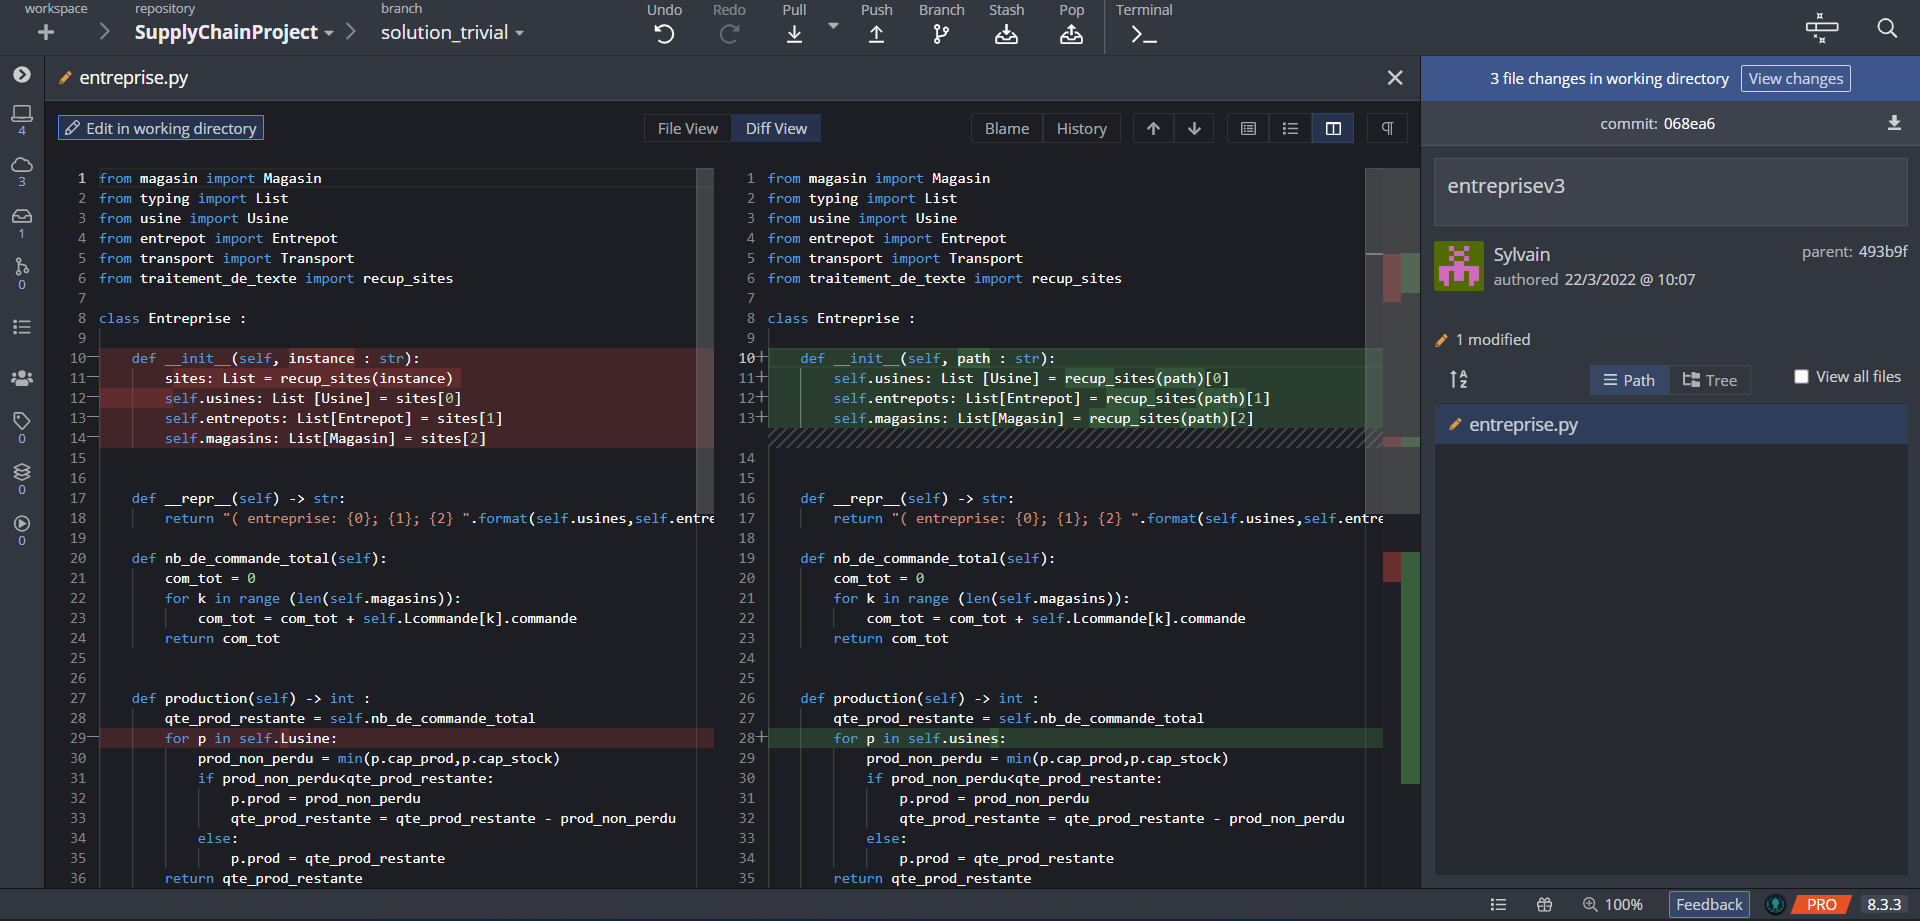
\includegraphics[width=1\textwidth]{gitkraken} % inclure l'image
    \caption{Split view de Gitkraken} % ajoute une légende
    \label{fig:gitkraken} % crée un label pour pouvoir y faire référence plus tard
\end{figure}


\noindent Le lien vers le dépôt du code est \emph{\href{https://github.com/mistertot/SupplyChainProject}{disponible ici}}.

\newpage

%************************************************************%

\section{Conception logicielle}
%----------------------------%
\subsection{Modèle objet}

\subsubsection{Classes}
Nous avons fait le choix de diviser chaque entité en une classe. La classe \emph{Site} recense les attributs communs des trois lieux (usines, entrepôts et magasins). Nous avons privilégié l'utilisation de l'héritage proposé par Python en utilisant l'initialisation avec \emph{build}. Nous avons pu ainsi créer trois classes filles à partir de la classe mère Site.
\begin{itemize}
\item La classe \emph{Usine}
\item La classe \emph{Entrepot}
\item La classe \emph{Magasin}
\end{itemize}

Par ailleurs, nous avons créé une classe \emph{Transport} qui modélise le transport d'un site i vers un site j. Comme il ne s'agit pas d'un site, nous n'avons pas utilisé d'héritage pour la construire.

De même, nous avons construit une classe \emph{Entreprise} qui comporte les méthodes principales de résolution du problème. Cette classe comporte une liste de sites, donc une liste d'usines, d'entrepôts et de magasins. Elle contient également les informations nécessaires à la résolution du problème, comme l'horizon de planification, le prix et toutes les données récupérées depuis les fichiers d'instances.

Enfin, la classe \emph{Probleme} fournie joue le rôle du chef d'orchestre de toutes les autres. C'est elle qui sera appelée pour la résolution du problème.

\subsubsection{Auxiliaires}
\begin{itemize}
\item \emph{traitement\_de\_texte} : Ce fichier comporte toutes les méthodes afin de réaliser tout le travail de lecture des différents fichiers \emph{nom-*.txt}. Il est utilisé dans le programme principal.
\item \emph{generateur\_de\_demandes} comporte toutes les méthodes de génération de demandes.
\end{itemize}

%----------------------------%
\subsection{Structure de données}

Les classes \emph{Usine}, \emph{Entrepot} et \emph{Magsin} sont définies comme filles de la classe \emph{Site}. Même si peu de méthodes sont rajoutées dans les classes \emph{Entrepot} et \emph{Magsin} en particulier, l'utilisation de l'héritage permet toutefois d'assurer la clarté et la logique du code, notamment lors de différents appels de ces classes.

La classe \emph{Site} comporte tous les attributs que peuvent contenir l'un des trois sites :
\begin{itemize}
\item La capacité de production
\item Le coût de production
\item La capacité de stockage
\item Le coût de stockage
\item Le stock initial
\item Le stock final
\end{itemize}
Ainsi, pour les sites ne comprenant pas certains de ces attributs, il est nécessaire de définir ces-derniers comme égaux à 0. Cela permet d'assurer une cohérence notamment avec la lecture des fichiers (notamment \emph{nom-site.txt}).

%************************************************************%

\section{Stratégie de résolution}

%----------------------------%
\subsection{Stratégie}
Dans un premier temps, nous avons modélisé une solution simple, la production se basant sur la somme des moyennes des demandes. Nous avons choisi de répartir cette production de manière linéaire : l'usine n°1 produit en premier dans la limite de sa capacité sans perte, puis l'usine n°2 et ainsi de suite.

Dans un second temps, nous avons voulu mettre en place une meilleure solution en comparant les coûts de l'ensemble des chemins possibles pour chaque magasin. Notre nouvelle méthode consistait à classer les coûts par ordre croissant puis à construire un quadruplet \emph{(usine, entrepôt, magasin, coût)}. A partir de ce classement il est alors possible de déterminer la quantité envoyée entre les sites sans perte.

%----------------------------%
\subsection{Algorithmes principaux}

\subsubsection{L'écriture}
L'algorithme d'écriture se trouve dans la classe \emph{Probleme}. Il se base sur le résultat de la méthode \emph{sol()} de la classe \emph{Entreprise}. Il crée un fichier \emph{nom.sol} dans le format demandé. La méthode \emph{sol()} est la méthode clef de la classe \emph{Entreprise} car elle renvoie le résultat sans mise en forme. Elle se base sur plusieurs autres méthodes de la classe \emph{Entreprise}. Nous allons nous pencher sur les principales.

\subsubsection{Classe Entreprise}
Comme nous l'avons évoqué précédemment, la classe \emph{Entreprise} comporte les méthodes principales.
La méthode :
\begin{itemize}
\item \emph{commande()} renvoie la demande prévisionnelle moyenne du magasin passé en argument (conformément à notre permière stratégie).
\item \emph{commande\_totale()} renvoie la somme des moyennes des demandes.
\item \emph{production()} se base sur notre stratégie de production. Pour chaque usine, elle calcule la quantité maxmimale qui peut être produite sans perte. Elle renvoie les quantités produites par chaque usine.
\item \emph{trans()} crée une matrice de taille $n\times n$ (n : nombre de sites). Selon la demande de chaque magasin, on transporte une certaine quantité. La logique est linéaire : le transport de la quantité produite vers la quantité demandée se fait dans l'ordre des usines et des magasins.
\item \emph{liste\_com()} renvoie les commandes prévues pour chaque magasin
\item \emph{cout\_prod\_tot()} renvoie le coût total de production du jour
\item \emph{stock\_sites()} rend compte de l'état des stocks de chaque site jour après jour
\item \emph{cout\_total\_stock()} renvoie le cout total du stock du jour 
\item\emph{cout\_trans()} renvoie le cout total de transport du jour
\end{itemize}

%************************************************************%

\section{Bilan}
%----------------------------%
\subsection{Résultats numériques}
En exécutant le fichier \emph{checker.py} pour l'instance \emph{A3b}, nous obtenons les résultats suivants :

\begin{figure}[h] % h pour here (ci-dessous)
    \centering
    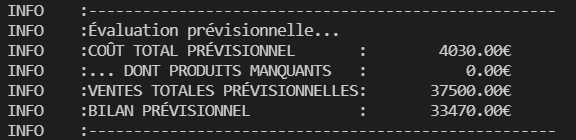
\includegraphics[width=1\textwidth]{checker} % inclure l'image
    \caption{Résultat pour l'instance A3b} % ajoute une légende
    \label{fig:checker} % crée un label pour pouvoir y faire référence plus tard
\end{figure}

Les résultats obtenus sont le reflet de notre première solution : comme celle-ci réagit de manière linéaire et sans recul, nous obtenons des bilans qui peuvent parfois poser problème. De plus, notre programme met nettement plus de temps à s'exécuter que les 10 secondes exigées. Malgré tout, nous parvenons à obtenir des résultats pour chaque instance.
%----------------------------%
\subsection{Limites et améliorations possibles}
Notre première solution a pu être correctement implémentée et fonctionne. En revanche, cette méthode ne permet pas d'aboutir à de bonnes combinaisons entre sites car elle est triviale.

Notre seconde idée n'a pu être implémentée dans les délais mais nous forgions en elle un espoir de gestion efficace des flux. Nous pouvions la situer à la frontière entre solution acceptable et solution optimale. Cependant, la comparaison des coûts de l'ensemble des chemins possibles pour chaque magasin aurait engendré une grande complexité algorithmique. Nous aurions dû ajouter des méthodes de tri efficaces telles que le tri fusion.

%************************************************************%
\end{document}